\documentclass[a4paper, 14pt]{article}
\usepackage{tocloft}

\usepackage{amsthm}
\newtheorem{theorem}{Теорема}
\newtheorem{lemma}{Лемма}

\usepackage{arxiv}

\usepackage[T2A]{fontenc}
\usepackage[utf8]{inputenc}
\usepackage[english, russian]{babel}
% \usepackage{cmap}
\usepackage{url}
\usepackage{booktabs}
\usepackage{nicefrac}
\usepackage{microtype}
\usepackage{lipsum}
\usepackage{graphicx}
\usepackage{subfig}
\usepackage[square,sort,comma,numbers]{natbib}
\usepackage{doi}
\usepackage{multicol}
\usepackage{multirow}
\usepackage{tabularx}
\usepackage{color,colortbl} % Раскраска таблицы
\definecolor{Gray}{gray}{0.9}

\usepackage{tikz}
\usetikzlibrary{matrix}

% Algorithms
\usepackage{algpseudocode}
\usepackage{algorithm}

%% Шрифты
\usepackage{euscript} % Шрифт Евклид
\usepackage{mathrsfs} % Красивый матшрифт
\usepackage{extsizes} % Возможность сделать 14-й шрифт

\usepackage{makecell} % diaghead in a table
\usepackage{amsmath,amsfonts,amssymb,amsthm,mathtools,dsfont}
\usepackage{icomma}

\newcommand{\bz}{\mathbf{z}}
\newcommand{\bx}{\mathbf{x}}
\newcommand{\by}{\mathbf{y}}
\newcommand{\bv}{\mathbf{v}}
\newcommand{\bw}{\mathbf{w}}
\newcommand{\ba}{\mathbf{a}}
\newcommand{\bb}{\mathbf{b}}
\newcommand{\bp}{\mathbf{p}}
\newcommand{\bq}{\mathbf{q}}
\newcommand{\bt}{\mathbf{t}}
\newcommand{\bu}{\mathbf{u}}
\newcommand{\bs}{\mathbf{s}}
\newcommand{\bT}{\mathbf{T}}
\newcommand{\bX}{\mathbf{X}}
\newcommand{\bZ}{\mathbf{Z}}
\newcommand{\bS}{\mathbf{S}}
\newcommand{\bH}{\mathbf{H}}
\newcommand{\bW}{\mathbf{W}}
\newcommand{\bY}{\mathbf{Y}}
\newcommand{\bU}{\mathbf{U}}
\newcommand{\bQ}{\mathbf{Q}}
\newcommand{\bP}{\mathbf{P}}
\newcommand{\bA}{\mathbf{A}}
\newcommand{\bB}{\mathbf{B}}
\newcommand{\bC}{\mathbf{C}}
\newcommand{\bE}{\mathbf{E}}
\newcommand{\bF}{\mathbf{F}}
\newcommand{\bomega}{\boldsymbol{\omega}}
\newcommand{\btheta}{\boldsymbol{\theta}}
\newcommand{\bgamma}{\boldsymbol{\gamma}}
\newcommand{\bdelta}{\boldsymbol{\delta}}
\newcommand{\bPsi}{\boldsymbol{\Psi}}
\newcommand{\bpsi}{\boldsymbol{\psi}}
\newcommand{\bxi}{\boldsymbol{\xi}}
\newcommand{\bchi}{\boldsymbol{\chi}}
\newcommand{\bzeta}{\boldsymbol{\zeta}}
\newcommand{\blambda}{\boldsymbol{\lambda}}
\newcommand{\beps}{\boldsymbol{\varepsilon}}
\newcommand{\bZeta}{\boldsymbol{Z}}
% mathcal
\newcommand{\cX}{\mathcal{X}}
\newcommand{\cY}{\mathcal{Y}}
\newcommand{\cW}{\mathcal{W}}

\newcommand{\dH}{\mathds{H}}
\newcommand{\dR}{\mathds{R}}
% transpose
\newcommand{\T}{^{\mathsf{T}}}

% \renewcommand{\shorttitle}{\textit{arXiv} Шаблон}
\renewcommand{\epsilon}{\ensuremath{\varepsilon}}
\renewcommand{\phi}{\ensuremath{\varphi}}
\renewcommand{\kappa}{\ensuremath{\varkappa}}
\renewcommand{\le}{\ensuremath{\leqslant}}
\renewcommand{\leq}{\ensuremath{\leqslant}}
\renewcommand{\ge}{\ensuremath{\geqslant}}
\renewcommand{\geq}{\ensuremath{\geqslant}}
\renewcommand{\emptyset}{\varnothing}

\usepackage{hyperref}
% \usepackage[usenames,dvipsnames,svgnames,table,rgb]{xcolor}

\hypersetup{
	unicode=true,
	pdftitle={A template for the arxiv style},
	pdfsubject={q-bio.NC, q-bio.QM},
	pdfauthor={David S.~Hippocampus, Elias D.~Striatum},
	pdfkeywords={First keyword, Second keyword, More},
	colorlinks=true,
	linkcolor=black,        % внутренние ссылки
	citecolor=blue,         % на библиографию
	filecolor=magenta,      % на файлы
	urlcolor=blue           % на URL
}

\graphicspath{{../figures/}}

\usepackage{enumitem} % Для модификаций перечневых окружений

\theoremstyle{definition} % "Определение"
\newtheorem{definition}{Опр.}[section]

\usepackage{etoolbox}

\makeatletter
\expandafter\patchcmd\csname\string\algorithmic\endcsname{\itemsep\z@}{\itemsep=1.5mm}{}{}
\makeatother
%%% Титульный лист
% \thispagestyle{empty}

\begin{titlepage}
    \begin{center}
        \textsc{Московский физико-технический институт}\\
        (национальный исследовательский университет)\\
        \textsc{Физтех-школа прикладной математики и информатики}\\
        \textsc{Кафедра интеллектуальных систем}
        \end{center}
        \vspace{1.5cm}
        \begin{center}
        {Никитина Мария Александровна}
        \par
        \vspace{2cm}
        {\Large \textsc{\textbf{Анализ смещения распределений при использовании сравнительного подхода в обучении представлений данных}}}
        \par
        \vspace{2cm}
        {03.03.01~--- Прикладные математика и физика}
        \par
        \vspace{1.5cm}
        \textsc{Выпускная квалификационная работа бакалавра}
        \end{center}
        \vspace{1.5cm}
        \hfill\parbox{8,4cm}{\textbf{Научный руководитель:}
        \\к.ф.-м.н. Р.\,В.\,Исаченко}
        \par
        \vspace{2.5cm}
        \begin{center}
        {Москва~--- 2024}
    \end{center}
\end{titlepage}
% \setcounter{page}{2}

\renewcommand{\abstractname}{Аннотация}

\title{Анализ смещения распределений при использовании сравнительного подхода в обучении представлений данных}

\author{
    Мария Никитина \\
	\texttt{nikitina.mariia@phystech.edu} \\
	\And
 	Роман Исаченко \\
	\texttt{roman.isachenko@phystech.edu}
}
\date{\today}

\begin{document}
% \maketitle
\thispagestyle{empty}

\begin{titlepage}
    \begin{center}
        \textsc{Московский физико-технический институт}\\
        (национальный исследовательский университет)\\
        \textsc{Физтех-школа прикладной математики и информатики}\\
        \textsc{Кафедра интеллектуальных систем}
        \end{center}
        \vspace{1.5cm}
        \begin{center}
        {Никитина Мария Александровна}
        \par
        \vspace{2cm}
        {\Large \textsc{\textbf{Анализ смещения распределений при использовании сравнительного подхода в обучении представлений данных}}}
        \par
        \vspace{2cm}
        {03.03.01~--- Прикладные математика и физика}
        \par
        \vspace{1.5cm}
        \textsc{Выпускная квалификационная работа бакалавра}
        \end{center}
        \vspace{1.5cm}
        \hfill\parbox{8,4cm}{\textbf{Научный руководитель:}
        \\к.ф.-м.н. Р.\,В.\,Исаченко}
        \par
        \vspace{2.5cm}
        \begin{center}
        {Москва~--- 2024}
    \end{center}
\end{titlepage}
\setcounter{page}{2}

\begin{abstract}
Среди подходов обучения без учителя contrastive learning в последнее время снова приобретает популярность. Данный метод заключается в сравнении пар из выборки для получения пространства представления, в котором похожие элементы как положительные будут находится близко, а отличающиеся -- далеко, как отрицательные. Однако наличие ложноотрицательных и ложноположительных пар вследствие шумов и погрешностей разметки приводит к смещению функции потерь, не учитывающей наличия таких элементов. В данной работе анализируются различные способы устранения этих искажений с целью точнее восстановить исходное распределение данных. Основываясь на примере из области обучения с учителем, разрабатывется несмещённая модель contrastive learning, исследуются её свойства. Качество несмещённого представления оценивается в задаче классификации, в задаче Image-Text retrieval, а также в искусственном эксперименте на примере двумерного пространства.
\end{abstract}

\keywords{Contrastive learning \and Representation learning \and Self-supervised learning}

\newpage
% \pagenumbering{roman} % use lowercase Roman numerals for page numbering before the main content

\tableofcontents
\clearpage % start the table of contents on a new page

% \pagenumbering{arabic}

\section{Введение}

Методы обучения без учителя становятся достаточно популярными в последнее время. Они хороши тем, что не требуют предварительной разметки данных, а, значит, для них можно проще и быстрее найти большие по объёму выборки для обучения.

\textit{Self-supervised learning} -- класс методов машинного обучения, позволяющих модели обучаться на задачах, которые не требуют явной разметки данных. Вместо этого используются некоторые характеристики выборки для создания своей собственной разметки. Часто такие методы используются для предварительной обрабоки датасета перед обучением с учителем.

В частности, \textit{representation learning} -- это процесс отображения необработанных входных данных в пространство векоторов-признаков или тензоров с целью найти и извлечь полезные закономерности, которые помогут в предсказании целевых значений.

При создании первых моделей машинного обучения много усилий тратилось на разработку методов преобразования данных и предварительной обработки, а модель использовалась только для принятия поверхностных решений на основе извлеченных признаков. Поэтому одной из ключевых составляющих успеха глубокого обучения является способность изучать и извлекать некоторые полезные признаки из данных. Увеличение объема доступных вычислений и размеченных датасетов позволило перейти от использования средств извлечения признаков, разработанных вручную, к автоматическому выделению особенностей. В результате исследования также сместились с разработки признаков на разработку архитектуры модели, которая самостоятельно может создавать представление данных.

К сожалению, задача поиска хорошего представления может быть сложной. Согласно \citep{LeKhac2020}, существует несколько принципов, на которых строится representation learning: выразительность и способность кодировать экспоненциальное число конфигураций в отличие от методов наподобие one-hot, абстрактность и отсутствие сильной зависимости от локальных небольших изменений, непротиворечивость и обеспечение наглядности представления. Одно из подходящих решений -- \textit{contrastive learning} -- подход при котором обучение происходит не только по принципу близости, но и по принципу различия. В отличие от дискриминативной модели, которая учится моделировать границу принятия решений среди классов, и генеративной модели, которая реконструирует входные выборки, при contrastive learning представление изучается путем сравнения пар элементов. Положим вектор $\textbf{x}$ некоторого объекта в качестве основного. Тогда вектор схожего объекта назовём $\textbf{x}^+$ -- позитивный элемент. Он должен быть как можно ближе к $\textbf{x}$ в пространстве эмбеддингов. А вектор отличного объекта $\textbf{x}^-$ -- как можно дальше, как негативный элемент. Основной сложностью использования такого подхода является правильный подбор негативных примеров на неразмеченных данных.

Существует две меры различия элементов: \textit{triplet loss} \citep{Schroff2015} и его модификация для $N$ негативных примеров -- \textit{Multi-Class N-pair loss} \citep{Sohn2016ImprovedDM}, а также \textit{Information Noise-Contrastive Estimation} или \textit{InfoNCE} \citep{Oord2018RepresentationLW} как обобщение N-pair loss.

Triplet loss был впервые использован в задаче распознавания одного и того же человека в разных позах и под разным углом. Пусть есть элемент $\mathbf{x}$. Выбирается один положительный элемент $\textbf{x}^+$ и один отрицательный $\textbf{x}^-$ с предположением, что $\textbf{x}^+$ принадлежит к тому же классу, что и $\mathbf{x}$, а $\mathbf{x}^-$ -- к другому. Затем расстояние между $\mathbf{x}$ и $\mathbf{x}^+$ уменьшается, а расстояние между $\mathbf{x}$ и $\mathbf{x}^-$ увеличивается:

\begin{equation}
    \mathcal{L}_{triplet}(\textbf{x}, \textbf{x}^+, \{\textbf{x}_i^-\}) = \sum\limits_{x \in \chi}\max(0, ||f(\textbf{x} - f(\textbf{x}^+)||_2^2 - ||f(\textbf{x} - f(\textbf{x}^-)||_2^2 + \epsilon
\end{equation}

Ввиду того, что обычно в качестве положительной пары берётся аугментация того же изображения, а в качестве отрицательной -- весь остальной батч, существует обобщение triplet loss на N негативных элементов:

\begin{equation}\label{eq:103}
    \mathcal{L}_{N-pair}(\textbf{x}, \textbf{x}^+, \{\textbf{x}_i^-\}_{i=1}^{N-1}; f) = - \log \frac{\exp(f(\textbf{x})^T f(\textbf{x}_i^+))}{\exp(f(\textbf{x})^T f(\textbf{x}_i^+)) + \sum _{i=1}^{N-1} \exp(f(\textbf{x})^Tf(\textbf{x}_i^-))}
\end{equation}

Если вместо $\exp(f(\textbf{x})^T f(\textbf{c}))$ брать любую функцию, аппроксимирующую $\frac{p(\textbf{x}|\textbf{c})}{p(\textbf{x})}$, получится InfoNCE loss:

\[\mathcal{L}_{InfoNCE} = -\mathbb{E}\left[\log\frac{f(\textbf{x}, \textbf{c})}{\sum_{\mathbf{x}' \in X}f(\textbf{x}', \textbf{c})}\right]\]

Методы contrastive learning хорошо себя показали в формировании визуальных представлений. Например, в \citep{chen2020simple} представлен фреймворк SimCLR, значительно превосходящий предыдущие self-supervised и semi-supervised методы. Его авторы разработали NT-Xent, в котором используется косинусное расстояние вместо скалярных произведений:

\[\mathcal{L}_{SimCLR}^{(i, j)} = - \log\frac{\exp(\text{sim}(g(\mathbf{h}_i), g(\mathbf{h}_j) / \tau)}{\sum\limits_{i \neq k}^{2N}\exp(\text{sim}(g(\mathbf{h}_i), g(\mathbf{h}_k) / \tau)},\]

\noindent где $\mathbf{h}_i = f(\mathbf{x})$, то есть вместо пространства представлений в лосс входит его проекция.

Во время обучения отсутствие истинных меток часто приводит к необходимости случайного выбора отрицательных экземпляров $\mathbf{x}^-$ из данных обучения. Однако такой подход приводит к смещению, если $\mathbf{x}^-$ на самом деле похож на $\mathbf{x}$. Это смещение приводит к значительному снижению качества\citep{NEURIPS2021_de8aa43e}.

В \citep{chuang2020debiased} предложен несмещённый контрастивный лосс. Учитывается $N$ отрицательных и $M$ положительных элементов из выборки. $L^{N, M}_{\text{DebiasedNeg}}(f)$ - функция потерь, которая корректирует ложноотрицательные экземпляры. Чтобы избавиться от необходимости разметки, элементы берутся из распределения данных, а положительное распределение создаётся искусственно с помощью аугментаций, которые могут содержать ложноположительные выбросы.

Эта работа направлена на разработку нового алгоритма для снижения вероятности смещения при появлении ложноположительных и ложноотрицательные элементов, а также оценку качества восстановления исходного распределения данных.

\newpage
\section{Предыдущие исследования}
Основная задача данного исследования -- создание пространства эмбеддинов, восстанавливающего начальное распределение, из которого были порождены данные. Идея учёта смещения в лосс-функции путём введения скрытых классов и вероятностей получить для элементов $\textbf{x}$ и $\textbf{x}^+$ один и тот же класс описана в \citep{chuang2020debiased} и \citep{Arora2019ATA}. В качестве распределения в скрытом пространстве берётся равномерное в предположении, что темы в лучшем пространстве эмбеддингов должны быть распределены таким образом. Рассматривается задача классификации на неразмеченных данных. В таком случае важно подобрать для $\textbf{x}$ отрицательные пары. Ввиду того, что в качестве положительных пар берутся различные аугментации данного изображения, а в качестве отрицательных -- все остальные картинки в батче, получается, что неизбежно появятся ложноотрицательные пары, так как не все изображения в выборке имеют класс, отличный от класса элемента $\textbf{x}$. В \citep{chuang2020debiased} в лосс-функции вероятность получить отрицательную пару выражается через полную вероятность и вероятность получить положительную пару. Тем самым приближается неизвестное распределение отрицательных элементов в выборке.

В \citep{ALBEF} и \citep{TCL} рассматривается применение contrastive learning в задаче сопоставления картинок и текстов для предобучения. В \citep{ALBEF} InfoNCE loss используется не только для сопоставления похожих картинок к картинкам, а текстов к текстам, но и для приближения эмбеддингов близких по смыслу картинок и текстов в одном пространстве перед тем, как передать их мультимодальной модели. Однако, в \citep{TCL}, в отличие от \citep{ALBEF}, также учитывается проблема того, что обычно в изображении хранится больше информации, чем описано в тексте. В \citep{TCL} применяется локальное выравнивание для максимизации взаимной информации между локальным и глобальным представлениями. Итоговая функция потерь в данном фреймворке состоит из кросс-модального выравнивания, где InfoNCE loss применяется для сравнения картинки с текстом и текста с картинкой:

\begin{equation}
    \mathcal{L}_{nce}(I, T_+, \{T_k\}_{k=1}^K) = - \mathbb{E}_{p(I, T)}\left[\log\frac{e^{(\text{sim}(I, T_+)/\tau)}}{\sum_{k=1}^Ke^{(\text{sim}(I, T_k)/\tau)}}\right],
\end{equation}

\noindent где $\tau$ -- параметр температуры, $T_+$ -- положительный текстовый семпл, $\{T_k\}_{k=1}^K$ -- множество негативных текстовых семплов, $\text{sim}(I, T_k) = f_v(v)^\top \hat{f}_t(\hat{t})$, где $f_v$ и $\hat{f}_t$ -- проекции выходов визуального и текстового энкодеров на пространство, в котором применяется лосс-функция. Для выбора отрицательных текстовых элементов используется идея, берущая начало с \textit{Memory Bank} \citep{MemoryBank}, который для уменьшения числа вычислений эмбеддингов хранит представления с предыдущих итераций. Эта идея имеет развитие в \citep{he2019moco}, где используются эмбеддинги не самой модели, а её версии с моментумом. Таким образом, $\hat{t}$ -- эмбеддинг, полученный с помощью модели с моментумом, а $\hat{f}_t$ -- функция, действующая на пространстве таких представлений. То есть параметры модели, вычисляющей хранимые эмбеддинги, представляют собой скользящее среднее по эпохам.

Аналогично определяется вторая часть данного лосса, высчитываемая относительно текста, а не изображения:

\begin{equation}
    \mathcal{L}_{nce}(T, I_+, \{I_k\}_{k=1}^K) = - \mathbb{E}_{p(I, T)}\left[\log\frac{e^{(\text{sim}(T, I)/\tau)}}{\sum_{k=1}^Ke^{(\text{sim}(T, I_k)/\tau)}}\right],
\end{equation}

\begin{equation}\label{eq:cma}
    \mathcal{L}_{cma} = \frac{1}{2}[\mathcal{L}_{nce}(I, T_+, \{T_k\}_{k=1}^K) + \mathcal{L}_{nce}(T, I_+, \{I_k\}_{k=1}^K)]
\end{equation}

Помимо кросс-модального сравнения, итоговая функция потерь включает в себя
внутри-модальное выравнивание, где InfoNCE loss применяется для сравнения картинки с картинкой и текста с текстом. Это используется, так как объекты разной модальности зачастую не могут полностью описать друг друга. В таком случае нужно выравнивание ещё и внутри каждой модальности, чтобы приблизить друг к другу различные аугментации одно и того же элемента данных:

\begin{equation}\label{eq:imc}
    \mathcal{L}_{imc} = \frac{1}{2}[\mathcal{L}_{nce}(T, T_+, \{T_k\}_{k=1}^K) + \mathcal{L}_{nce}(I, I_+, \{I_k\}_{k=1}^K)]
\end{equation}

Для того, чтобы учитывать не только глобальную информацию с изображений и текста, в итоговую функцию потерь в \citep{TCL} входит локальная максимизация, где с помощью InfoNCE loss часть изображения сравнивается со всем изображением, а часть текста -- со всем текстом:

\begin{equation}\label{eq:lmi}
    \mathcal{L}_{lmi} = \frac{1}{2}\left[\frac{1}{M}\sum\limits_{i=1}^M\mathcal{L}_{nce}(T, T_+^i, \{T_k\}_{k=1}^K) + \frac{1}{N}\sum\limits_{j=1}^N\mathcal{L}_{nce}(I, I_+^j, \{I_k\}_{k=1}^K)\right],
\end{equation}

\noindent где $T^i$ -- $i$-ая часть изображения, $I^j$ -- $j$-ая часть текста.

Чтобы соединить представления картинок и изображений, используется задача бинарной классификации, где в качестве таргета используется результат применения лосса из кросс-модального выравнивания, а в качестве предсказания -- выход полносвязного слоя общего энкодера:

\begin{equation}
    \mathcal{L}_{itm} = \mathbb{E}_{p(I, T)}H(\phi(I, T), y^{(I, T)}),
\end{equation}

\noindent где $H(;)$ -- кросс-энтропия, $y^{(I, T)}$ -- таргет.

Маскированная текстовая модель, в которой слова с вероятностью 15\% заменяются на специальный токен [MASK] или случайное слово, используется для того, чтобы снизить влияние шума. Предсказание пропущенного слова основывается на контексте текста и изображения:

\begin{equation}
    \mathcal{L}_{mlm} = \mathbb{E}_{p(I, T^{msk})}H(\Phi(I, T^{msk}), y^{T^{msk}}),
\end{equation}

\noindent где $\Phi(I, T^{msk})$ -- предсказанная вероятность $T^{msk}$, $y^{T^{msk}}$ -- настоящий токен.

Итоговый лосс в \citep{TCL}:

\begin{equation}
    \mathcal{L} = \mathcal{L}_{cma} + \mathcal{L}_{imc} + \mathcal{L}_{lmi} + \mathcal{L}_{itm} + \mathcal{L}_{mlm}
\end{equation}

Обоснование применения InfoNCE заключается в том, что он связан с нижней границей взаимной информации, которую тяжело посчитать напрямую. В \citep{Oord2018RepresentationLW} представлено доказательство этого факта с помощью связи лосса с MINE \citep{belghazi2021mine}.

\newpage
\section{Постановка задачи}

\subsection{Несмещённый лосс}

Пусть $\mathcal{X}$ -- предметное пространство. Contrastive learning работает с семантически близкими парами точек $(\mathbf{x}, \mathbf{x}^+)$, где $\mathbf{x}$ берётся из распределения данных $p(x)$ над $\mathcal{X}$. Цель состоит в том, чтобы найти функцию эмбеддинга $f: \mathcal{X} \rightarrow \mathbb{R}^d$. В \citep{chuang2020debiased} предполагается, что существует множество дискретных скрытых классов $\mathcal{C}$ и положительные пары $(\mathbf{x}, \mathbf{x}^+)$ имеют один и тот же класс. Распределение по $\mathcal{C}$ обозначается $\rho(c)$, следовательно, совместное
распределение $p_{x,c}(\textbf{x}, c) = p(\textbf{x}|c)\rho(c)$. Пусть $h : \mathcal{X} \rightarrow \mathcal{C}$ -- функция, присваивающая метки классов. Тогда $p^+_x(\textbf{x}') = p(\textbf{x}'|h(\textbf{x}') = h(\textbf{x}))$ -- вероятность сказать, что $\textbf{x}'$ -- положительная пара для $\textbf{x}$, и $p^-_x(\textbf{x}') = p(\textbf{x}'|h(\textbf{x}') \neq h(\textbf{x}))$ -- для отрицательной пары. Предполагается, что вероятности классов $\rho(\textbf{x}) = \tau^+$ однородны и $\tau^- = 1 - \tau^+$ -- ворятность обнаружить любой другой класс. Тогда «идеальный» лосс при условии наличия $N$ негативных элементов выглядеть так:

\begin{equation}\label{eq:1}
\mathcal{L}_{\text{Unbiased}}^N(f) = \mathbb{E}_{\substack{\textbf{x} \sim p, \textbf{x}^+ \sim p^+_x,\\ \textbf{x}_i^- \sim p_x^-}} \bigg[-\log \frac{e^{f(\textbf{x})^T f(\textbf{x}^+)}}{e^{f(\textbf{x})^T f(\textbf{x}^+)} + \sum _{i=1}^N e^{f(\textbf{x})^T f(\textbf{x}_i^-)}}\bigg]
\end{equation}

На практике $p_x^-(\textbf{x}_i^-)$ неизвестно, поэтому $\textbf{x}_i^-$ выбирается из немаркированного распределения $p(\textbf{x})$. С вероятностью $\tau^+$ попадётся ложноотрицательный элемент. Лосс для такого случая уже будет смещённым.

\begin{equation}\label{eq:2}
\mathcal{L}_{\text{Biased}}^N(f) = \mathbb{E}_{\substack{\textbf{x} \sim p, \textbf{x}^+ \sim p^+_x,\\ \textbf{x}_i^- \sim p_x}} \bigg[-\log \frac{e^{f(\textbf{x})^T f(\textbf{x}^+)}}{e^{f(\textbf{x})^T f(\textbf{x}^+)} + \sum _{i=1}^N e^{f(\textbf{x})^T f(\textbf{x}_i^-)}}\bigg]
\end{equation}

В \citep{chuang2020debiased} доказывается лемма о том, что в пределе при $N \to \infty$ лосс функция $L_{\text{Biased}}^N(f)$ является верхней гранью $L_{\text{Unbiased}}^N(f)$.

Распределение $p(\mathbf{x})$ при условии наличия $M$ положительных элементов можно разложить:

\begin{equation}\label{eq:3}
p(\textbf{x}') = \tau^+ p^+_x(\textbf{x}') + \tau^-p_x^-(\textbf{x}')
\end{equation}

Выразим $p^-_x(\textbf{x}')$:

\begin{equation} \label{eq:4}
p_x^-(\textbf{x}') = \frac{p(\textbf{x}') - \tau^+ p^+_x(\textbf{x}')}{\tau^-}
\end{equation}

Подсчёт $p^-_x(\textbf{x}')$ через $p(\mathbf{x})$ и $p^+_x(\textbf{x}')$ в итоговой формуле очень дорогостоящий. Поэтому в \citep{chuang2020debiased} предлагается использовать приближение итоговой функции потерь:

\begin{equation}\label{eq:5}
\mathcal{L}_{\text{Neg}}^{N, M}(f) = \mathbb{E}_{\substack{\textbf{x} \sim p; \textbf{x}_+ \sim p_x^+,\\ \{\textbf{u}_i\}_{i=1}^N \sim p^N \\ \{\textbf{v}_j\}_{j=1}^M \sim {p_x^+}^M}}  \bigg[ -\log \frac{e^{f(\textbf{x})^T f(\textbf{x}^+)} }{e^{f(\textbf{x})^T f(\textbf{x}^+)} + N g\big(\textbf{x}, \{\textbf{u}_i\}_{i=1}^N, \{\textbf{v}_j\}_{j=1}^M\big)} \bigg],
\end{equation}

\noindent где эмпирическая оценка $p(\mathbf{x}^-)$:

\begin{equation}\label{eq:6}
g\big(\textbf{x}, \{\textbf{u}_i\}_{i=1}^N, \{\textbf{v}_j\}_{j=1}^M\big) = \max \bigg\{ \frac{1}{\tau^-}\bigg(\frac{1}{N} \sum \limits_{i=1}^N e^{f(\textbf{x})^T f(\textbf{u}_i)} - \tau^+ \frac{1}{M} \sum \limits_{j=1}^M e^{f(\textbf{x})^T f(\textbf{v}_j)}\bigg), e^{-1/t}\bigg\}.
\end{equation}

$\{\textbf{u}_i\}_{i=1}^N$ -- $N$ сэмплов из $p(\mathbf{x'})$ и $\{\textbf{v}_j\}_{j=1}^M$ -- $M$ сэмплов из $p(\mathbf{x'}^+)$, $t$ -- параметр температуры.

% В \citep{chuang2020debiased} также приводится оценка скорости сходимости $L_{\text{Neg}}^{N, M}(f)$ к случаю бесконечного $N$ и $M = 1$:

% \begin{equation}\label{eq:102}
% |\tilde{L}_{\text{DebiasedNeg}}^N(f) - L_{\text{DebiasedNeg}}^{N, M}(f)| \leq \frac{e^{3/2}}{\tau^-}\sqrt{\frac{\pi}{2N}} + \frac{e^{3/2}\tau^+}{\tau^-}\sqrt{\frac{\pi}{2M}}
% \end{equation}

Применение данной лосс-функции в модели SimCLR позволило смоделировать смещение при наличии в выборке ложноотрицательных элементов и увеличить точность результата. В данной работе будет произведено её сравнение с лосс-функцией, в которой вместо $p(\mathbf{x}^-)$ будет выражен $p(\mathbf{x}^+)$.

\subsection{Ложноположительные элементы}

Чрезмерная аугментация в попытке получить как можно большее $M$ приводит к появлению ложноположительных сэмплов и смещению оценки. Оценим распределение положительных элементов в рамках функции потерь.

\begin{equation}\label{eq:7}
p_x^+ (\textbf{x}') = \frac{p(\textbf{x}') - \tau^- p^-_x(\textbf{x}')}{\tau^+}
\end{equation}

\begin{lemma}
% \normalfont 
При $N \to \infty$:
\begin{equation} \label{eq:8}
\begin{split}
\mathcal{L}_{\text{Unbiased}}^N(f) = \mathbb{E}_{\substack{\textbf{x} \sim p \\ \textbf{x}^+ \sim p_x^+ \\ \{\textbf{x}_i^-\}_{i=1}^N \sim {p_x^-}^N}} \bigg[ - \log \frac{e^{f(\textbf{x})^T f(\textbf{x}^+)}}{e^{f(\textbf{x})^T f(\textbf{x}^+)} + \sum_{i=1}^N e^{f(\textbf{x})^T f(\textbf{x}_i^-)}} \bigg] \longrightarrow \\
\longrightarrow \mathbb{E}_{\substack{\textbf{x} \sim p \\ \textbf{x}^- \sim p_x^-}} \bigg[ - \log \frac{R}{R + N \mathbb{E}_{\textbf{x}^- \sim p_x^-} e^{f(\textbf{x})^T f(\textbf{x}^-)}} \bigg],
\end{split}
\end{equation}

\noindent где
\begin{equation}\label{eq:9}
R = \frac{1}{\tau^+} \big(\mathbb{E}_{\textbf{x}' \sim p} e^{f(\textbf{x})^T f(\textbf{x}')} - \tau^- \mathbb{E}_{\textbf{x}^- \sim p_x^-} e^{f(\textbf{x})^T f(\textbf{x}^-)}\big).
\end{equation}
\end{lemma}

\renewcommand\qedsymbol{$\blacksquare$}
\begin{proof}
Поскольку выражение внутри математического ожидания ограничено, мы можем применить теорему Лебега о мажорируемой сходимости:

\begin{equation}
\begin{split}
\lim_{N \to \infty} \mathbb{E} \bigg[ - \log \frac{e^{f(\textbf{x})^T f(\textbf{x}^+)}}{e^{f(\textbf{x})^T f(\textbf{x}^+)} + \sum_{i=1}^N e^{f(\textbf{x})^T f(\textbf{x}_i^-)}} \bigg] = \\
= \mathbb{E} \bigg[ \lim_{N \to \infty} - \log \frac{e^{f(\textbf{x})^T f(\textbf{x}^+)}}{e^{f(\textbf{x})^T f(\textbf{x}^+)} + \sum_{i=1}^N e^{f(\textbf{x})^T f(\textbf{x}_i^-)}} \bigg] = \\
= \mathbb{E} \bigg[ - \log \frac{\mathbb{E}_{\textbf{x}^+ \sim p_x^+} e^{f(\textbf{x})^T f(\textbf{x}^+)}}{\mathbb{E}_{\textbf{x}^+ \sim p_x^+} e^{f(\textbf{x})^T f(\textbf{x}^+)} + N \mathbb{E}_{\textbf{x}^- \sim p_x^-} e^{f(\textbf{x})^T f(\textbf{x}^-)}}\bigg]
\end{split}
\end{equation}

Используя \ref{eq:7} и линейность матожидания, получим:

\[\mathbb{E}_{\textbf{x}^+ \sim p_x^+} e^{f(\textbf{x})^T f(\textbf{x}^+)} = \frac{1}{\tau^+} \big(\mathbb{E}_{\textbf{x}' \sim p} e^{f(\textbf{x})^T f(\textbf{x}')} - \tau^- \mathbb{E}_{\textbf{x}^- \sim p_x^-} e^{f(\textbf{x})^T f(\textbf{x}^-)}\big) = R.\]
\end{proof}

\subsection{Функция потерь $\mathcal{L}_{\text{Pos}}$}

Назовём предел в лемме $\tilde{\mathcal{L}}_{\text{Pos}}^N (f)$:

\begin{equation} \label{eq:10}
\tilde{\mathcal{L}}_{\text{Pos}}^N (f) = \mathbb{E}_{\substack{\textbf{x} \sim p \\ \textbf{x}^- \sim p_x^-}} \bigg[ - \log \frac{\mathbb{E}_{\textbf{x}' \sim p} e^{f(\textbf{x})^T f(\textbf{x}')} - \tau^- \mathbb{E}_{\textbf{x}^- \sim p_x^-} e^{f(\textbf{x})^T f(\textbf{x}_i^-)}}{\mathbb{E}_{\textbf{x}' \sim p} e^{f(\textbf{x})^T f(\textbf{x}')} + \big(N \tau^+ - \tau^-\big) \mathbb{E}_{\textbf{x}^- \sim p_x^-} e^{f(\textbf{x})^T f(\textbf{x}_i^-)}}\bigg]
\end{equation}

Полученная функция потерь при конечном $N$:

\begin{equation}\label{eq:11}
\mathcal{L}_{\text{Pos}}^N (f) = \mathbb{E}_{\substack{\textbf{x} \sim p \\ \{\textbf{u}_i\}_{i=1}^N \sim {p_x^-}^N \\ \textbf{v} \sim p_x^+}} \bigg[-\log \frac{P_{\text{emp}} (\textbf{x}, \{\textbf{u}_i\}_{i=1}^N, \textbf{v}) - \tau^- P_{\text{emp}}^- (\textbf{x}, \{\textbf{u}_i\}_{i=1}^N)} {P_{\text{emp}} (\textbf{x}, \{\textbf{u}_i\}_{i=1}^N, \textbf{v})+ \big(N \tau^+ - \tau^-\big) P_{\text{emp}}^- (\textbf{x}, \{\textbf{u}_i\}_{i=1}^N) }\bigg],
\end{equation}

\noindent где
\begin{equation} \label{eq:12}
P_{\text{emp}} (\textbf{x}, \{\textbf{u}_i\}_{i=1}^N, \textbf{v}) = \frac{1}{N+2} \bigg(\sum \limits_{i=1}^N e^{f(\textbf{x})^T f(\textbf{u}_i)} + e^{f(\textbf{x})^T f(\textbf{v})} + e^{f(\textbf{x})^T f(\textbf{x})}\bigg);
\end{equation}

\begin{equation} \label{eq:13}
P_{\text{emp}}^- (\textbf{x}, \{\textbf{u}_i\}_{i=1}^N) = \frac{1}{N} \sum \limits_{i=1}^N e^{f(\textbf{x})^T f(\textbf{u}_i)}.
\end{equation}

В \citep{Oord2018RepresentationLW} представлено доказательство того факта, что InfoNCE loss максимизирует нижнюю границу взаимной информации.

\begin{theorem}
\label{thm:asympt}
$\mathcal{L}_{\text{Pos}}$ максимизирует нижнюю границу взаимной информации.
\end{theorem}

\begin{proof}
Пусть $c$ -- контекст, $x$ -- элемент выборки. Тогда взаимная информация:

\[I(x, c) = \sum\limits_{x \in X, c \in C}p(x, c)\log \frac{p(x|c)}{p(x)}\]

Так как рассматриваемый лосс -- это категориальная кросс-энтропия классификации положительного сэмпла корректно, то оптимальная для него вероятность того, что $x_i$ -- положительный элемент:

\[p(x_i \text{ -- положительный} | X, x) = \frac{p(x_i|c)\prod_{l \neq i}p(x_l)}{\sum_{j=1}^Np(x_j|c)\prod_{l \neq j}p(x_l)} = \frac{\frac{p(x_i|c)}{p(x_i)}}{\sum_{j=1}^{N+1}\frac{p(x_j|c)}{p(x_j)}}\]

Так как в пределе при $N \to \infty$ лосс-функцию можно представить в виде:

\[\mathcal{L} = - \mathbb{E}_{x \in p}\left(\log\frac{f(x, c)}{\sum_{x_j \in X}f(x_j, c)}\right),\]

\noindent то $\frac{p(x_i|c)}{p(x_i)}$ -- оптимальное значение для $f(x_i, c)$. Тогда:

\[\mathcal{L}_{\text{Pos}} = \mathbb{E}_{\substack{x \sim p \\ x_i \sim p_x^-}} \bigg[ - \log \frac{\mathbb{E}_{x \sim p}f(x, c) - \tau^- \mathbb{E}_{x^- \sim p_x^-} f(x_i^-, c)}{\mathbb{E}_{x \sim p} f(x, c) + \big(N \tau^+ - \tau^-\big) \mathbb{E}_{x^- \sim p_x^-} f(x_i^-, c)}\bigg] =\]

\[= \mathbb{E}_{\substack{x \sim p \\ x_i^- \sim p_x^-}} \bigg[\log \frac{\mathbb{E}_{x \sim p}\frac{p(x|c)}{p(x)} + \big(N \tau^+ - \tau^-\big) \mathbb{E}_{x^- \sim p_x^-}\frac{p(x_i^-|c)}{p(x)}}{\mathbb{E}_{x \sim p}\frac{p(x|c)}{p(x)} - \tau^- \mathbb{E}_{x^- \sim p_x^-}\frac{p(x_i^-|c)}{p(x)}}\bigg] \approx\]

\[\approx \mathbb{E}_{\substack{x \sim p \\ x_i^- \sim p_x^-}} \bigg[\log \frac{\frac{1}{N + 2}\left(\frac{p(x|c)}{p(x)} + \sum\limits_{i=1}^N\frac{p(x_i^-|c)}{p(x_i^-)} + \frac{p(c|c)}{p(c)}\right) + \big(N \tau^+ - \tau^-\big)\frac{1}{N}\sum\limits_{i=1}^N\frac{p(x_i^-|c)}{p(x_i^-)}}{\frac{1}{N + 2}\left(\frac{p(x|c)}{p(x)} + \sum\limits_{i=1}^N\frac{p(x_i^-|c)}{p(x_i^-)} + \frac{p(c|c)}{p(c)}\right) - \tau^-\frac{1}{N}\sum\limits_{i=1}^N\frac{p(x_i^-|c)}{p(x_i^-)}}\bigg] \approx\]

\[\approx \mathbb{E}_{\substack{x \sim p \\ x_i^- \sim p_x^-}} \bigg[\log \frac{\frac{p(x|c)}{p(x)} + N\mathbb{E}_{x_i^- \sim p_x^-}\frac{p(x_i^-|c)}{p(x_i^-)} + 1 + \big(N \tau^+ - \tau^-\big)(N + 2)\mathbb{E}_{x_i^- \sim p_x^-}\frac{p(x_i^-|c)}{p(x_i^-)}}{\frac{p(x|c)}{p(x)} + N\mathbb{E}_{x_i^- \sim p_x^-}\frac{p(x_i^-|c)}{p(x_i^-)} + 1 - \tau^-(N + 2)\mathbb{E}_{x_i^- \sim p_x^-}\frac{p(x_i^-|c)}{p(x_i^-)}}\bigg] =\]

\[= \mathbb{E}_{x \sim p}\bigg[\log \frac{\frac{p(x|c)}{p(x)} + N + 1 + N^2\tau^+ + 2N\tau^+ - N\tau^- - 2\tau^-}{\frac{p(x|c)}{p(x)} + N + 1 - (N + 2)\tau^-}\bigg] =\]

\[= \mathbb{E}_{x \sim p}\log \bigg[1 + \frac{N(N + 2)\tau^+}{\frac{p(x|c)}{p(x)} + N\tau^+ + 1 - 2\tau^-}\bigg] = \mathbb{E}_{x \sim p}\log \bigg[1 + \frac{N(N + 2)\tau^+\frac{p(x)}{p(x|c)}}{1 + \left(N\tau^+ + 1 - 2\tau^-\right)\frac{p(x)}{p(x|c)}}\bigg] \geq\]

\[\geq \mathbb{E}_{x \sim p}\log \bigg[\frac{N(N + 2)\tau^+\frac{p(x)}{p(x|c)}}{1 + \left(N\tau^+ + 1 - 2\tau^-\right)\frac{p(x)}{p(x|c)}}\bigg] =\]

\[= - I(x, c) + \mathbb{E}_{x \sim p}\log \bigg[\frac{N(N + 2)\tau^+}{1 + \left(N\tau^+ + 1 - 2\tau^-\right)\frac{p(x)}{p(x|c)}}\bigg] =\]

\[= - I(x, c) + \mathbb{E}_{x \sim p}\log \bigg[\frac{(N + 2)\tau^+}{\frac{1}{N} + \left(\tau^+ + \frac{1}{N} - \frac{2\tau^-}{N}\right)\frac{p(x)}{p(x|c)}}\bigg]\]

При $N \to \infty$ получим:

\[- I(x, c) + \mathbb{E}_{x \sim p}\log \bigg[\frac{(N + 2)\tau^+}{\frac{1}{N} + \left(\tau^+ + \frac{1}{N} - \frac{2\tau^-}{N}\right)\frac{p(x)}{p(x|c)}}\bigg] \geq - I(x, c) + \mathbb{E}_{x \sim p}\log \bigg[\frac{(N + 2)\tau^+}{\tau^+\frac{p(x)}{p(x|c)}}\bigg] \geq\]

\[\geq - I(x, c) + \mathbb{E}_{x \sim p}\log\left((N + 2)\frac{p(x|c)}{p(x)}\right)\]

Следовательно,

\[I(x, c) \geq \mathbb{E}_{x \sim p}\log\left((N + 2)\frac{p(x|c)}{p(x)}\right) - \mathcal{L}_{\text{Pos}}\]

При условии того, что $\frac{p(x|c)}{p(x)}$ задаётся распределением данных в выборке и не зависит от $N$, получаем, что первое слагаемое в выражении справа при $N \to \infty$ больше нуля.

\end{proof}

\newpage
\section{Вычислительный эксперимент}

\subsection{Классификация}
В первом вычислительном эксперименте проводится сравнение $\mathcal{L}_{N-pair}$ (\ref{eq:103}) и $\mathcal{L}_{\text{Pos}}^N(f)$ (\ref{eq:11}) в задаче классификации изображений. В качестве датасета используется CIFAR10 \citep{krizhevsky2009learning}, состоящий из 60000 цветных изображений размером 32x32 для классификации. Бейзлайн-модель: SimCLR \citep{chuang2020debiased} с энкодером ResNet18 \citep{he2015deep} и N-pair loss (\ref{eq:103}), оптимизатор -- Adam \citep{kingma2017adam}, learning rate 0.001, размер батча 256. Все модели тренируются 50 эпох и оцениваются линейным классификатором после получения эмбеддинга.

Сравнение результатов работы можно увидеть на рис.\ref{fg:acc1}-\ref{fg:acc5}. В качестве метрики берётся топ-1 и топ-5 accuracy:

\[Acc_1 = \frac{TP + TN}{TP + FP + TN + FN}\]

\[Acc_k = \frac{1}{n}\sum\limits_{i=1}^n[y_i \in \hat{y}_i^k]\]

\begin{figure}[!ht]
    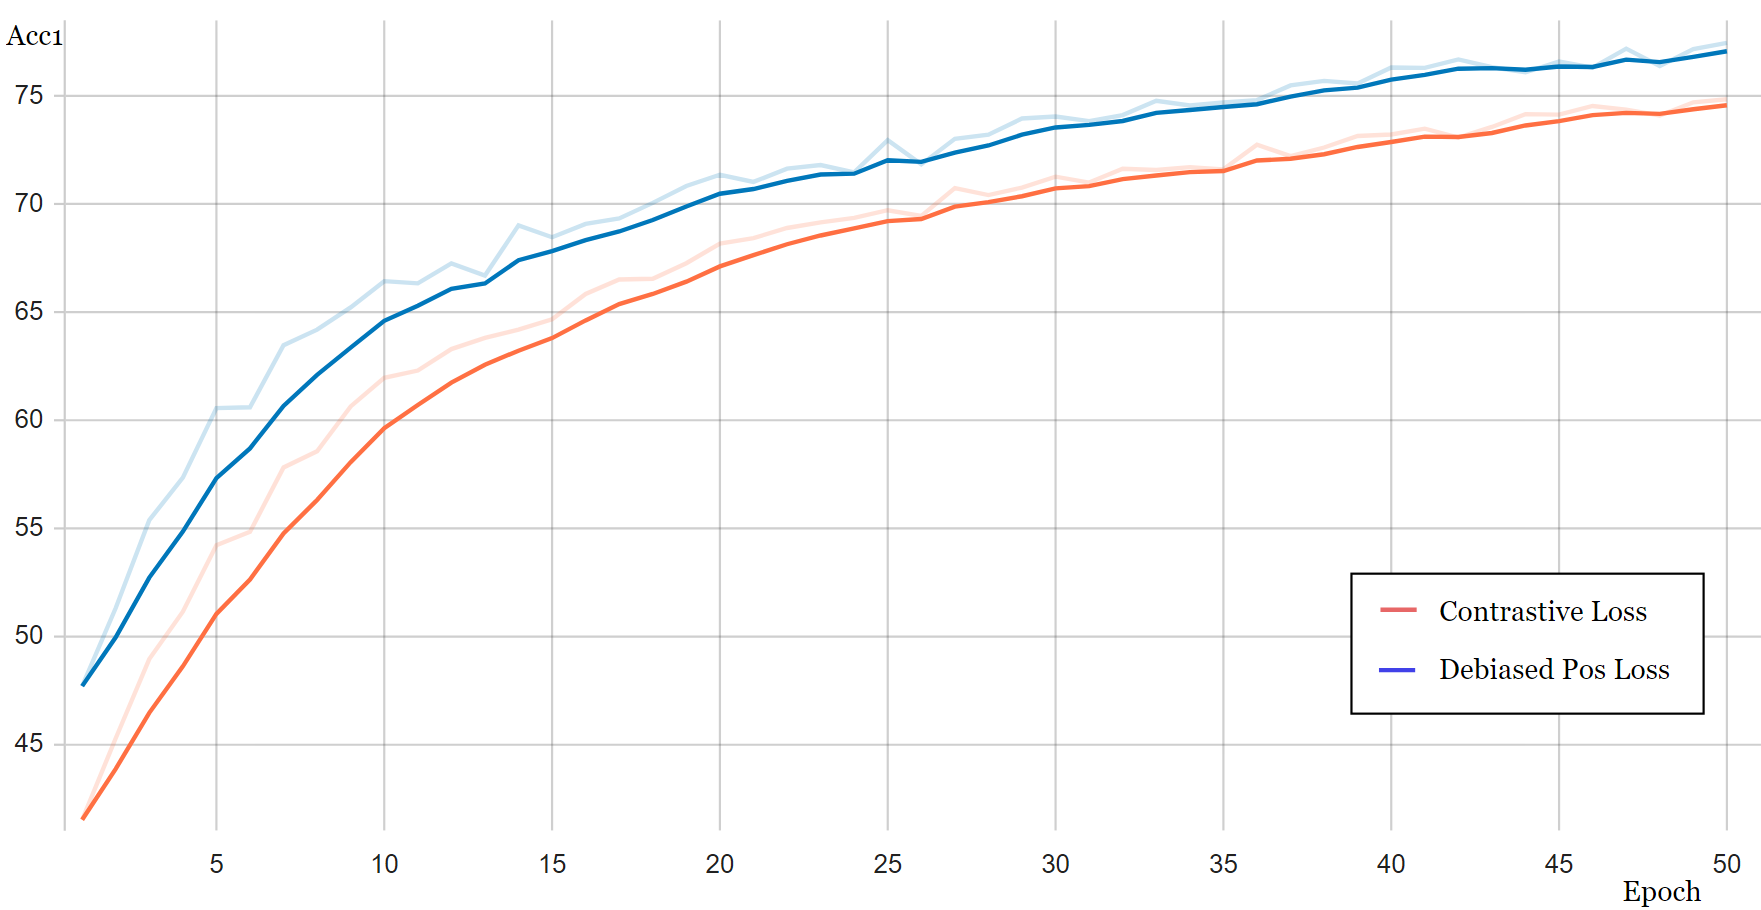
\includegraphics[scale = 0.45]{Pictures/loss_acc1.png}
    \caption{Метрика acc1 классификации с использованием N-pair loss и DebiasedPos loss.}
    \label{fg:acc1}
\end{figure}

\begin{figure}[!ht]
    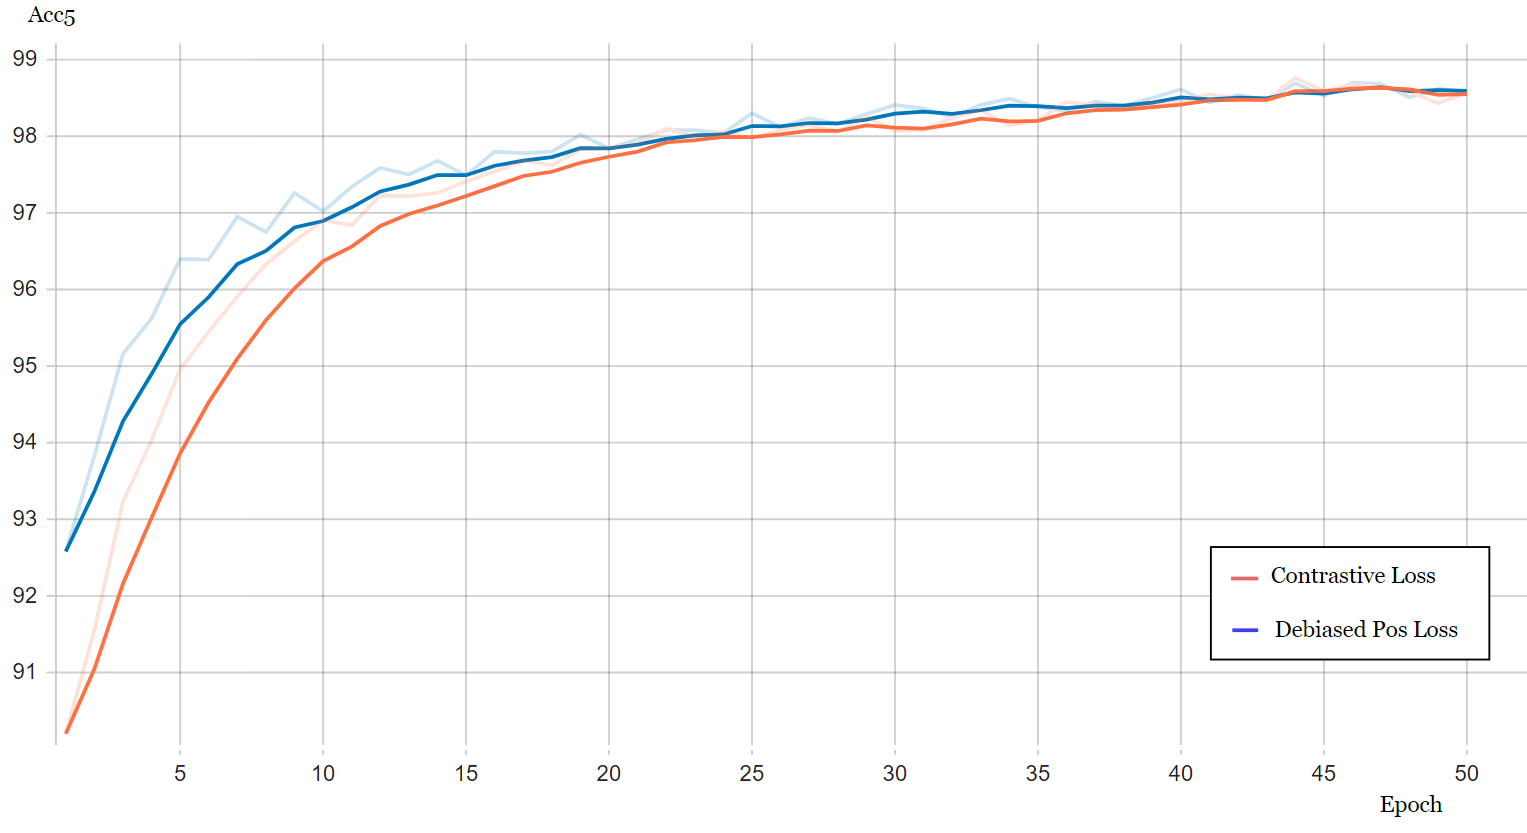
\includegraphics[scale = 0.52]{Pictures/loss_acc5.png}
    \caption{Метрика acc5 классификации с использованием N-pair loss и DebiasedPos loss.}
    \label{fg:acc5}
\end{figure}

Как видно, модель, использующая $\mathcal{L}_{\text{Pos}}^N(f)$ имеет метрику топ-1 accuracy на $3.5\%$ лучше. Топ-5 accuracy по истечении 50 эпох у моделей одинаковая, однако для модели с $\mathcal{L}_{\text{Pos}}^N(f)$ метрика растёт быстрее.

\subsection{Искусственный эксперимент}
Одна из задач данной работы -- анализ пространства представления, порождённого предложенной лосс-функцией. Для этого генерируется стандартное нормальное распределение $\mathbf{z}$ в качестве изначальных данных, затем создаётся две модели нормализующего потока, которые каждый вектор $\mathbf{z}$ переводят в вектор, заданный некоторым другим распределением. В качестве таких распределений взяты moons и blobs из библиотеки sklearn. Полученные из одного и того же $\mathbf{z}$ вектора $\mathbf{a}$ и $\mathbf{b}$ подаются на вход энкодеру, состоящему из двух полносвязных слоёв.

Лосс-функция делится на две части: первая отвечает за сближение векторов, порождённых из одного и того же изначального вектора -- это $\mathcal{L}_{N-pair}$, $\mathcal{L}_{Neg}$ или $\mathcal{L}_{Pos}$. Так как они используют косинусное расстояние, выходы энкодеров нормируются перед подсчётом лосс-функции. Вторая часть -- приближение итогового распределения к нормальному. Так как contrastive loss имеет несколько локальных минимумов и не обязательно каждый из них описывает нормальное распределение, для выхода каждого энкодера подсчитывается следующая функция потерь: из среднего по батчу и его дисперсии генерируется нормальное распределение, которое с помощью дивергенции Кульбака-Лейблера сравнивается со стандартным нормальным распределением.

\begin{figure}[!ht]
    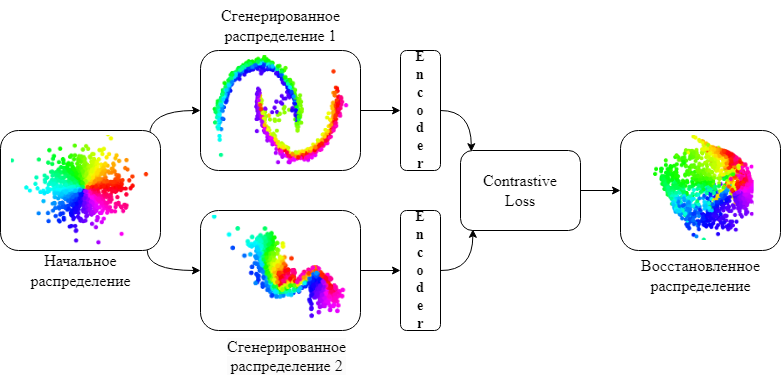
\includegraphics[scale = 0.65]{Pictures/Model.png}
    \caption{Схема модели искусственного эксперимента. Точки одинакового цвета получены из одной и той же точки начального распределения.}
    \label{fg:model}
\end{figure}

\subsection{VQA}
В качестве большого эксперимента на реальных данных взята задача Visual Question Answering \citep{VQA}. Датасет состоит из 204 721 картинок из MS COCO \citep{lin2015microsoft}, 760 000 вопросов и около 10 миллионов ответов. Бейзлайн модель -- TCL \citep{TCL} с лосс-функцией $\mathcal{L} = \mathcal{L}_{cma} + \mathcal{L}_{imc} + \mathcal{L}_{lmi} + \mathcal{L}_{itm} + \mathcal{L}_{mlm}$. Все сравниваемые модели дообучаются с предложенной авторами \citep{TCL} предобученной модели при замороженном визуальном энкодере 5 эпох на 100 000 вопросах и оценивается на 50 000 вопросах. В качестве метрики используется accuracy, которая равна 1, если ответ модели находится в предложенном авторами VQA списке из 10 ответов для каждого вопроса.

Новые модели создаются посредством замены $\mathcal{L}_{N-pair}$ в $\mathcal{L}_{cma}$ (\ref{eq:cma}), $\mathcal{L}_{imc}$ (\ref{eq:imc}), $\mathcal{L}_{lmi}$ (\ref{eq:lmi}) на $\mathcal{L}_{Pos}$ и $\mathcal{L}_{Neg}$. В качестве метрики берётся число попаданий ответа модели в список из 10 ответов, предоставленных составителями датасета:

\[Acc = \frac{1}{n}\sum\limits_{i = 1}^n[y_i \in y_i^{10}]\]

Результаты представлены в таблице \ref{res_vqa}.

\begin{table}
\begin{center}
\caption{Результаты VQA для $\mathcal{L}_{N-pair}$ и $\mathcal{L}_{Pos}$}
\begin{tabular}{| c | c | c |}
\hline
& $\mathcal{L}_{N-pair}$ & $\mathcal{L}_{Pos}$ \\ \hline
Accuracy & 0.67 & 0.69 \\ \hline
\end{tabular}
\label{res_vqa}
\end{center}
\end{table}

\begin{figure}[!ht]
    \begin{center}
    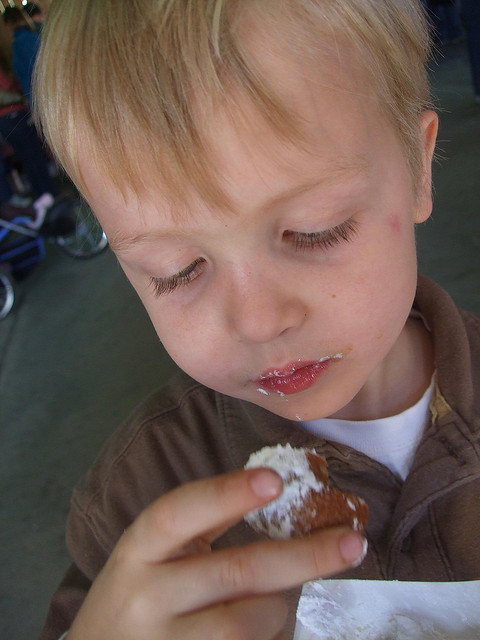
\includegraphics[scale = 0.45]{Pictures/contrastive_example.png}
    \caption{Пример работы модели в VQA-задаче. Вопрос: «What is the child eating?» Ответ модели с $\mathcal{L}_{Pos}$: «donut».}
    \label{fg:vqa}
    \end{center}
\end{figure}

\newpage
\section{Заключение}
В данной работы был проведён анализ смещения положительного и отрицательного распределения в задаче контрастного обучения на примере классификации изображений, искусственного двумерного эксперимента и VQA. Была предложена лосс-функция, учитывающая шум при сэмплировании положительных элементов, доказана её сходимость к $\mathcal{L}_{N-pair}$ и свойство максимизации правдоподобия между сравниваемыми положительными элементами.

\newpage
\bibliographystyle{plain}
\bibliography{references.bib}

\end{document}
